\chapter{Evaluation}\label{chap:evaluation}
Citation recommender systems are arguably more difficult to evaluate than other types of recommender systems. The evaluation depends heavily on the ground truths which are chosen. In this case, the ground truths are the papers \textit{actually cited} by the authors in the test citation contexts. So the task performed during evaluation is the task of re-prediction. 

However, this is a very subjective way of carrying out an evaluation. There is no reason to believe that all the test contexts' authors have cited the correct papers. Not all people who author papers are experienced researchers, so it is possible that they missed other suitable papers which might have been cited in the same place. What this means for the evaluation is that the citation results produced by the algorithms might actually be suitable even though they are not present in the ground truth. For this reason, it is important to conduct an online evaluation (user study) in conjunction with a normal offline evaluation. 

There is also the possibility that the test citation context might not have enough information necessary to make the prediction. It might be the case that the correct paper to cite becomes clear only after reading adjacent paragraphs in the paper. MAG, in particular, has a lot of citation contexts from which it is not possible to recommend any paper. This is a common problem which will bring down the metric scores, but that is the nature of the citation recommendation problem. 

The following section (6.1) gives a short description of the evaluation metrics used. Sections 6.2 and 6.3 describe the offline and online evaluation respectively.

\section{Evaluation Metrics}

Before calculating the metrics, the recommendations are binarized. For three of the metrics, this step assigns a '1' for a relevant recommendation (a paper in the ground truth) and a '0' for a recommendation which is not in the ground truth. 

The NDCG metric which will be described shortly assigns different relevance values to different relevant documents. This applies only in the case of Arxiv-MAG where we have considered one primary recommendation and other secondary recommendations. Here, a '2' is assigned for the primary recommendation, '1' is assinged for a secondary recommendations and '0' is assigned to recommended papers which are not part of the ground truth. In other words, primary recommendations are twice as important as secondary recommendations while calculating the NDCG.

It is important to note that the NDCG is not very useful when used with the other data sets which don't have graded ranks (such as MAG). While it is still reported for all the data sets, it is not a metric which we pay a lot of attention to.

In the following definitions, the word 'query' refers to a test set citation context for which recommendations are retrieved.

\textbf{Precision@k}: The precision@k gives the percentage of relevant documents in the top k recommendations for a single query. \\
Example: the binarized array [1, 0, 0, 1, 0] has precision@3=1/3, precision@5 = 2/5

\textbf{Average Precision (AP)}: Let $K_1,K_2,...,K_R$ be the ranks of each relevant document. The average precision for a query (test context) gives the average of precision@k values for $K_1,K_2,...,K_R$.\\
Example: the binarized array [1, 0, 0, 1, 0] has an average precision of $\frac{(1/1 + 2/4)}{2}$.

\textbf{Mean Average Precision (MAP)}: This is the first of the metrics that is reported for our data sets. The mean average precision is simply the mean of the average precision values over multiple queries (test set contexts).
Let the average precisions of the recommendations for all the n test set contexts are $AP_1, AP_2, AP3, ..., AP_n$. Then, 
\begin{equation*}
    MAP = \frac{\sum\limits_{i=1}^n AP_i}{n}
\end{equation*}
\textbf{Recall@k}:
Recall is a measure which gives the percentage of true positives found in the first k recommendations for a single query. 

While average precision averaged over queries is called mean average precision, Recall@k when averaged over queries, is still called Recall@k. This is a bit of a misnomer, but the term 'Recall@k' actually refers to the \textit{Average Recall@k} while evaluating recommender systems.
So in this thesis, Recall@k gives the average recall over all n test set contexts.
\begin{equation*}
    Recall = \frac{\sum\limits_{i=1}^n R_i}{n}
\end{equation*}
where R is the recall for a single test set context.
Example: Let there be 3 relevant items in the ground truth and two queries in the test set.
The binarized array [0,0,1,0,0] has a R@5 of 1/3. The binarized array [1,0,0,1,0] has a R@5 of 2/3. So the final Recall@5 = $\frac{(1/3 + 2/3)}{2}$

\textbf{Reciprocal Rank (RR)}:
The reciprocal rank is simply the reciprocal of the rank of a relevant item. 

\textbf{Mean Reciprocal Rank (MRR)}:
The MRR is obtained by averaging the reciprocal ranks over all queries. It is a metric which is most often used when there is only one relevant item. 
As the test sets in this thesis \textit{generally} have only one relevant item in the ground truth list, this is a useful metric. In cases where there is more than one relevant item in the ground truth list, only the  rank of the \textit{highest-ranked relvant item} is considered. 

Example: the MRR of the binarized arrays [0,1,0,1,0] and [0,0,1,0,0] is $\frac{(1/2 + 1/3)}{2}$. Only the reciprocal rank of the highest-ranked relevant item is used in the MRR calculation.

\textbf{Discounted Cumulative Gain (DCG@k)}:
This is a metric which assumes that relevant documents have different degrees of relevance. In this thesis, this only applies to the Arxiv-MAG data set, in which the primary recommendation gets a value of '2', and the secondary recommendations (if present) get a value of '1'. 

The 'gain' obtained from secondary recommendations is less (it is discounted) than the gain obtained from a primary recommendation.
There are different discounts used in DCG calculations. In this thesis, a discount of $1/log_2 i$ is applied (where i is the position of the rank).
The discounts applied are therefore [1.0, 1.0, 0.6309, 0.5, 0.4307, ...]. 

Let $rel(r_i)$ be the relevance score -- 0/1/2. Then,
\begin{equation*}
    DCG@k = \frac{rel(r_1)}{1} + \sum\limits_{i=2}^k \frac{rel(r_i)}{log_2 i}
\end{equation*}
where the denominator for i=1 is 1 (as $log_2 1 = 0$). 

The DCG when all the relevant items have the same importance (such as in MAG) discounts items of the same importance. As these items of same importance are ordered arbitrarily, the DCG (and consequently the NDCG) is a deceptive and unsuitable metric for data sets like MAG which don't have graded importance.

\textbf{Ideal DCG}:
The ideal DCG@k is calculated in this thesis by sorting the top 500 recommendations in descending order and calculating the DCG@k. Any relevant item below a rank of 500 is therefore not considered to be relevant. This means that a '2', if present in the top 500 ranks, will be at the head of the list of recommendations, and will be followed by 1's and 0s.

\textbf{Normalized Discounted Cumulative Gain (NDCG)}
The normalized discounted gain for a single query is obtained by dividing the DCG@k by the Ideal DCG@k. 
\begin{equation*}
    NDCG@k = \frac{DCG@k}{IDCG@k}
\end{equation*}
where IDCG is the Ideal DCG.

This is divided by the number of queries to get the final mean NDCG@k. 
As mentioned earlier, NDCG is not particularly a suitable metric for MAG, MAG50 and Unpaywall-MAG.
\section{Offline evaluation}
In this section, we will go through the offline evaluation, in which we use the data sets explained in Chapter 4 and the approaches explained in Chapter 5. The test sets used contain citation contexts only (and not the title, abstract or full text). Based on the data set, the training was done using either the full text or the title, abstract and citation contexts (pseudo full-text), or both. 

\subsection{Training and test sets}
The filter criteria used for the creating the training and test sets are given in Appendix~\ref{chap:offlineevalfilter}. Table~\ref{tab:trainingteststats} shows the number of test set contexts, number of training set papers and other details for all the data sets. 

\begin{table}[]
    \centering
    \begin{tabular}{lllrr}
    \toprule
       Data set  & Training Years & Test Years & \#Training Papers & \#Test Contexts \\
       \midrule
       ACL-MAG  & 1965-2005 & 2006 & 11,217 & 2,775 \\
       Arxiv-MAG  & 1991-2016 & 2017 & 376,218 & 286,272 \\
       Unpaywall-MAG  & $\le$2017 & 2018-2019 & 1,185,090 & 182,327 \\
       MAG  & 1800-2017 & 2018-2019 & 1,620,841 & 168,700 \\
       MAG50  & 1800-2017 & 2018-2019 & 126,666 & 107,781 \\
       MAG-Cited  & 1800-2017 & 2018-2019 & 1,478,924 & 190,991 \\
       \bottomrule
    \end{tabular}
    \caption{Details about Training and Test Sets}
    \label{tab:trainingteststats}
\end{table}

The number of training set papers has interesting ramifications for the evaluation results. In general, it is reasonable to expect that more complex algorithms perform better with more training examples. We can hypothesise that less complex algorithms might perform better with fewer training examples. The number of training examples varies widely across data sets, with ACL-MAG at the lower end and the regular MAG data set at the higher end. A bar graph of the number of training set papers is given in Figure~\ref{fig:trainingsetpapers}.\\
Apart from the algorithms themselves, the number of citation contexts in the test sets also have a big effect on the evaluation results. The more the number of test set contexts, the higher is the confidence we can have in the results. The training-test split is done based on years for all the data sets, as shown in Table~\ref{tab:trainingteststats}. The number of test set contexts from these papers varies widely too, with ACL-MAG by far the smallest data set in these terms, and Arxiv-MAG the largest (the ratio of test set contexts to training set papers for Arxiv-MAG is also the highest). However, all the other data sets have a large number of citation contexts too. The number of test set contexts per data set is shown in a bar graph in Figure~\ref{fig:testsetcontexts}. 

\begin{figure}
    \centering
    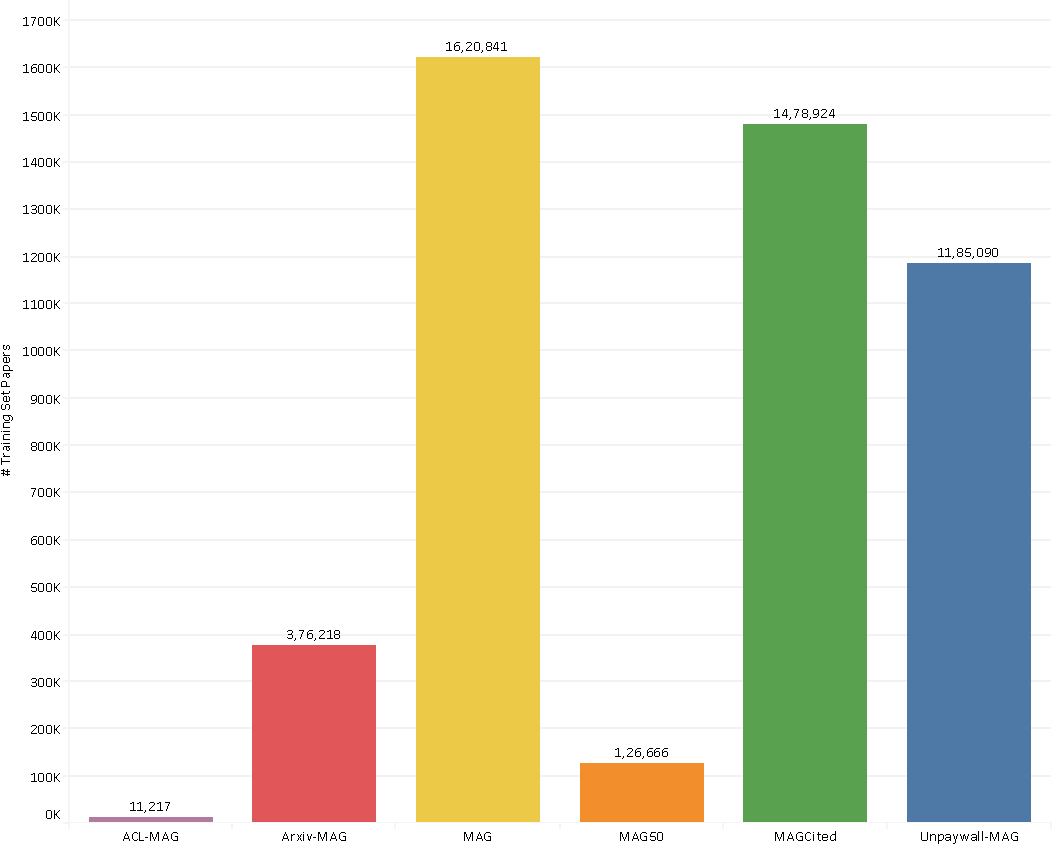
\includegraphics[width=10cm]{figures/Evaluation/trainingteststats.pdf}
    \caption{No. of training set papers per data set}
    \label{fig:trainingsetpapers}
\end{figure}
\begin{figure}
    \centering
    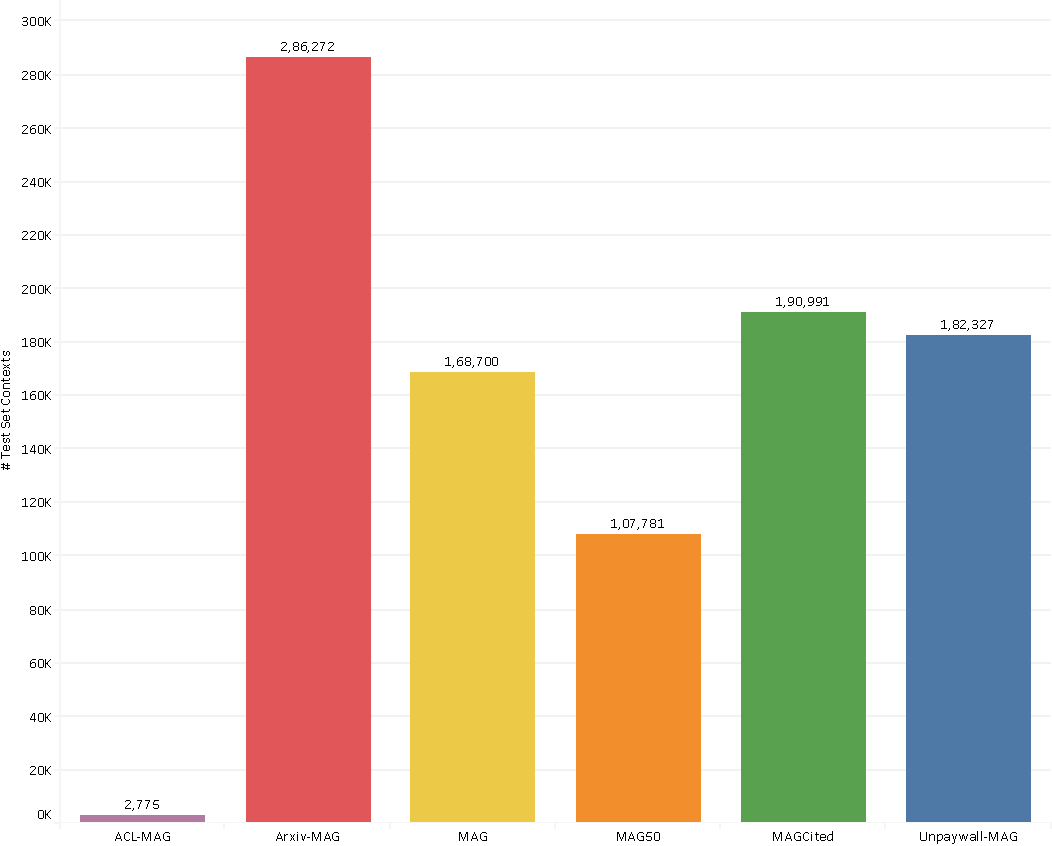
\includegraphics[width=10cm]{figures/Evaluation/testsetcontexts.pdf}
    \caption{No. of test set contexts per data set}
    \label{fig:testsetcontexts}
\end{figure}
\subsection{Offline evaluation across data sets}
Four metrics from Section 6.1 are used in the offline evaluation -- Recall, MRR, NDCG and MAP. Of these, NDCG is a useful metric only for data sets which have grading of relevant items -- where some items are 'more relevant' than others. The only two data sets which have graded relevant items are ACL-MAG and Arxiv-MAG. But none of the test set contexts for ACL-MAG actually have more than one relevant item. So the NDCG is mainly applicable for only Arxiv-MAG. However, it is reported for the other data sets as well even though we will not talk about it at all in relation to the MAG data sets where its values can be deceptive.

The Recall is probably the most important metric in citation recommendation as it gives the percentage of the ground truths which have been recommended. MAP is generally used along with Recall in evaluation of information retrieval and in citation recommendation systems, and is also reported here. It penalises false positives, while recall penalises false negatives. As a large majority of the test set contexts (across data sets) have only one relevant paper in the ground truth, the MRR is also an important metric. It describes the rank of the highest ranked paper in cases where there is more than one element in the ground truth. 

The evaluation is performed for: 
\begin{itemize}
    \item Embedding-based algorithms: Paper2Vec, Doc2Vec, hd2vOUT, hd2vINOUT (hyperdoc2vec with OUT document vectors, and both IN and OUT document vectors respectively).
    \item Information retrieval algorithm: BM25
    \item Topic Modelling algorithm: Variational Bayes LDA used as a baseline (LDA Mallet is included for ACL-MAG)
    \item Semi-genetic hybrid algorithm based on BM25 and hd2vOUT
\end{itemize}
\begin{table}[]
\centering
    \caption{Evaluation scores at k=10 for all models using the MAG data.}
    \label{tab:magevalk10}
\begin{center}
    \begin{tabular}{lllll}
    \toprule
    Model & MRR@10 & Recall@10 & MAP@10 & NDCG@10 \\
    \midrule
    hd2vOUT  & 0.0974 & 0.2149 & 0.0969 & 0.1430 \\
    BM25       & 0.1146 & 0.2098 & 0.1141 & 0.1540 \\
    hd2vINOUT & 0.0134 & 0.0194 & 0.0133 & 0.0167 \\
    Hybrid  & \textbf{0.1422} & \textbf{0.3087} & \textbf{0.1414} & \textbf{0.2051} \\
    LDA     & 0.0123 & 0.0307 & 0.0123 & 0.0192 \\
    Paper2Vec        & 0.0006 & 0.0020 & 0.0007 & 0.0011 \\
    Doc2Vec       & 0.0000008 & 0.000005 & 0.0000008 & 0.000006 \\
    \bottomrule
    \end{tabular}
\end{center}
\end{table}
\subsection{Evaluation of MAG data sets}
Figure~\ref{fig:magevaluation} shows the evaluation metrics for all the models tested using the MAG data set without any restriction on the number of citations. The evaluation results for all the models at k=10 using the MAG data set are given in Table~\ref{tab:magevalk10}.

It is clear from the graph and the table that the hybrid model has the best results using every metric. This is not a surprise as it combines the best parts of the next 2 best models, BM25 and hd2vOUT. While hd2vOUT has marginally higher recall, BM25 has slightly higher MRR and MAP. 
Unlike the other data sets we will look at shortly, hd2vINOUT performs very badly. This indicates that using the contexts and the abstract as pseudo full-text has not quite paid off in terms of the quality of IN embeddings. The much higher hd2vOUT values show that the OUT embeddings are of much better quality. The OUT embeddings correspond to the papers playing the role of a cited document, so this shows that Hyperdoc2vec is highly context-aware. 
\begin{figure}
    \centering
    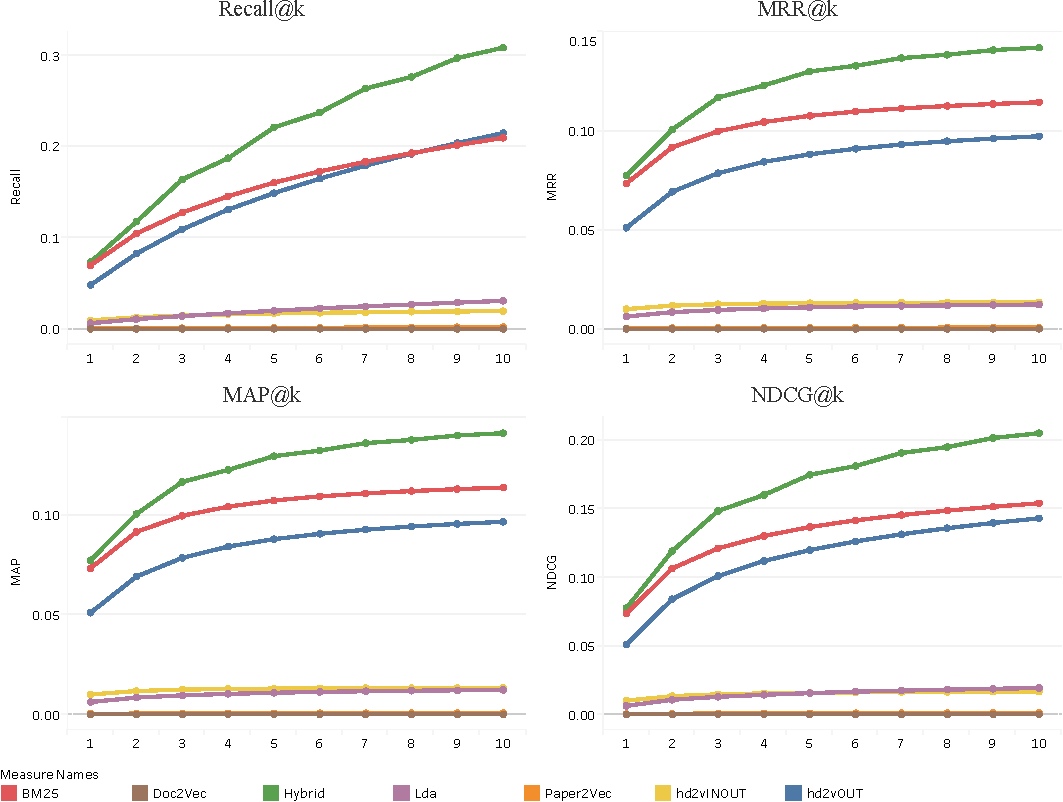
\includegraphics[keepaspectratio, width=.9\linewidth]{figures/Evaluation/MAGMetricsGraph.pdf}
    \caption{Evaluation using MAG}
    \label{fig:magevaluation}
\end{figure}

\begin{figure}
    \centering
    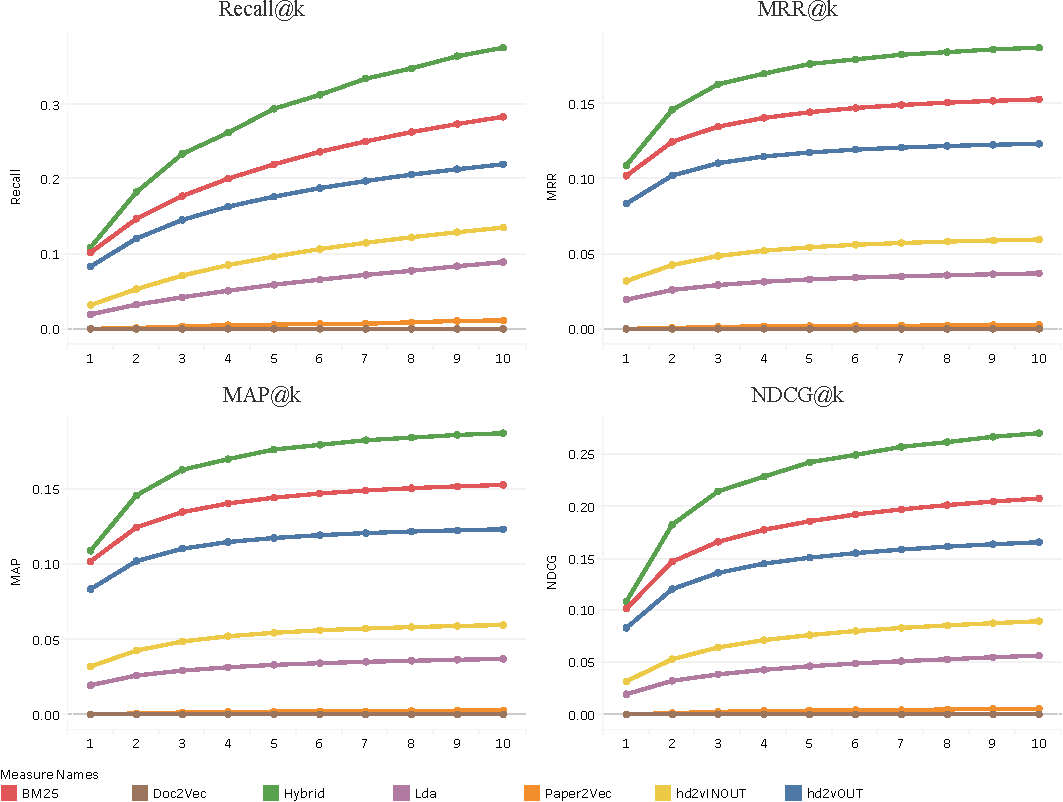
\includegraphics[keepaspectratio, width=.9\linewidth]{figures/Evaluation/MAG50MetricsGraph.pdf}
    \caption{Evaluation using MAG50: only papers with >= 50 citations in training set}
    \label{fig:mag50evaluation}
\end{figure}

The performance of LDA is below average, but it does better than hd2vINOUT for the MAG data set. Paper2Vec and Doc2Vec perform abysmally across metrics. While Paper2Vec is a lot better than Doc2Vec (the DeepWalk has clearly made a difference), it does not do a good job by any means.
\begin{table}[]
\centering
    \caption{Evaluation scores at k=10 for all models using the MAG50 data.}
    \label{tab:mag50evalk10}
\begin{center}
    \begin{tabular}{lllll}
    \toprule
    Model & MRR@10 & Recall@10 & MAP@10 & NDCG@10 \\
    \midrule
    hd2vOUT  & 0.1233 & 0.2200 & 0.1233 & 0.1660 \\
    BM25       & 0.1528 & 0.2836 & 0.1528 & 0.2082 \\
    hd2vINOUT & 0.0595 & 0.1353 & 0.1873 & 0.0898 \\
    Hybrid  & \textbf{0.1873} & \textbf{0.3760} & \textbf{0.1873} & \textbf{0.2711} \\
    LDA     & 0.0369 & 0.0892 & 0.0369 & 0.0567 \\
    Paper2Vec        & 0.0025 & 0.0113 & 0.0026 & 0.0055 \\
    \bottomrule
    \end{tabular}
\end{center}
\end{table}
Figure~\ref{fig:mag50evaluation} shows the evaluation results for all the models using the MAG50 data set -- MAG with the restriction that papers in the training set (which are to be be recommended) should have at least 50 citations. Only test set contexts with papers in the ground truth that have at least 50 citations are retained.

One would expect that MAG50 would produce better results for all the algorithms on all the metrics, and that is indeed the case at k=10 (see Table~\ref{tab:mag50evalk10}). All the metric values are significantly higher for all the data sets. This is because the data sets are of similar quality, but the number of candidates for each recommendation is much smaller for MAG50 than MAG. Consequently, it is more likely that the relevant items are near the top of the list of recommendations.  

However, the inference cannot be made that a system using MAG50 always produces better results. Less popular papers and very new papers are not recommended while using the MAG50 data set even though they may be perfectly valid recommendations. But some users might might want to be recommended only papers with a lot of citations in a running citation recommender system. So HybridCite, the final recommender system (described in Section 5.6), uses two models under the hood -- one using MAG data and the other using MAG50 data. 
\subsection{Case study using BM25 on 2 MAG data sets}
In this subsection, we perform a small case study to test the assertion made in Huang et al's two papers~\cite{HuangKCMGR12,Huang2015} that citation contexts describe the cited paper rather than the citing paper. This is done using the BM25 algorithm, which is best suited to prove this point.
\begin{figure}[h]
    \centering
    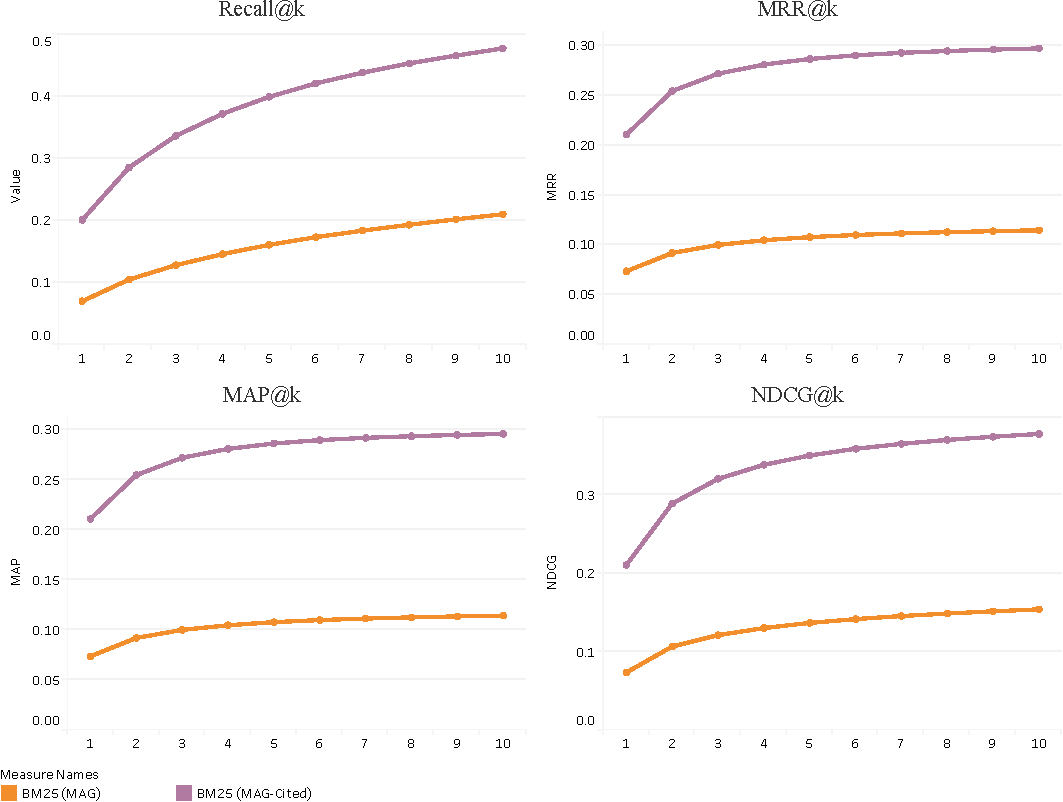
\includegraphics[keepaspectratio, width=.9\linewidth]{figures/Evaluation/MagCitedMetricGraphs.pdf}
    \caption{Comparison of BM25 Evaluation for 2 MAG data sets: MAG and MAG-Cited}
    \label{fig:magcitedevaluation}
\end{figure}
\begin{figure}
    \centering
    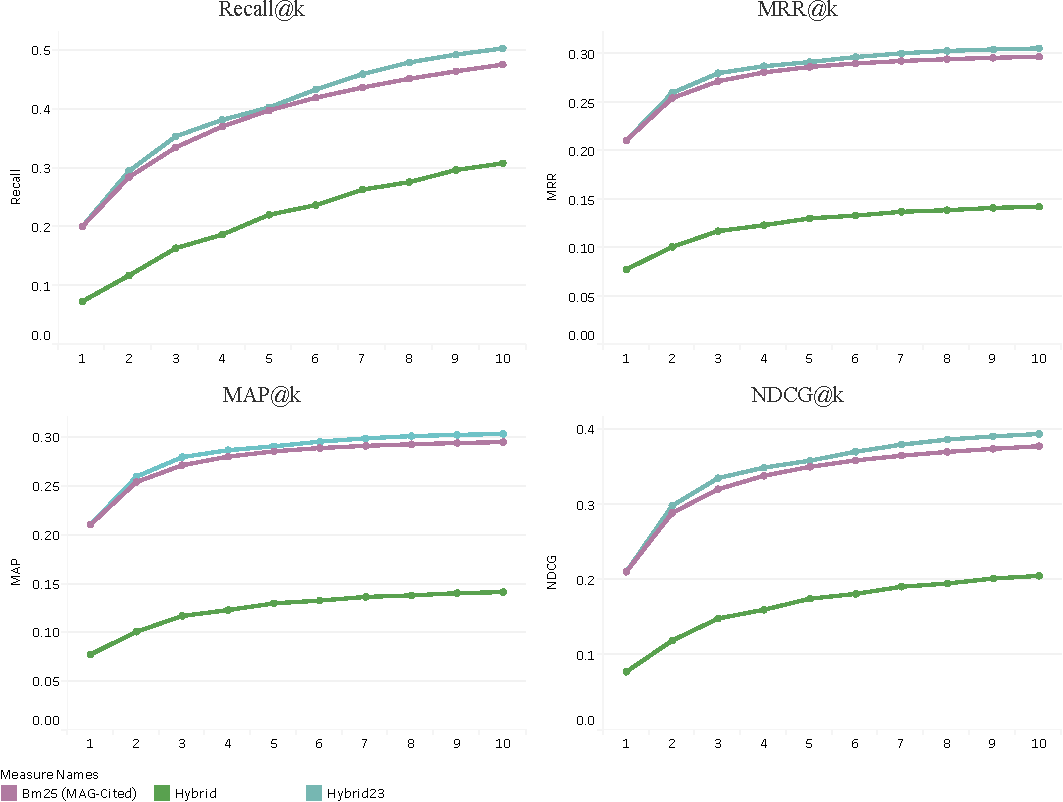
\includegraphics[keepaspectratio, width=.9\linewidth]{figures/Evaluation/MAGHybridv2metrics.pdf}
    \caption{Comparing Hybrid23 with BM25 (MAG-Cited) and the original Hybrid algorithm}
    \label{fig:maghybridevaluation}
\end{figure}
For the purpose of doing the case study, a new data set called MAG-Cited was created (the creation process is described in Section 4.2.6). The text for each paper is made up of its title, abstract and \textit{citation contexts from papers which cite it}. In other words, the content of a cited paper contains citation contexts from all its citing papers.
The text for each paper in the regular MAG data set, on the other hand, is made up of its title, abstract and citations contexts (i.e., citation contexts from its own content). 

Running the BM25 algorithm on both the data sets, we find that there is a very large difference in the evaluation results. The metrics show that using the citation contexts of a citing paper as the content of a cited paper pays off. The evaluation results are shown in Figure~\ref{fig:magcitedevaluation} and prove Huang et al's assertion pretty comprehensively. 

This result has the potential to improve recommendation results when used in a hybrid recommender system. So, an improved hybrid system (called Hybrid23) was built using two data sets and three components. The system in explained in Section 5.5.

As already explained, the Hybrid23 system retrieves recommendations from BM25 trained on the MAG data set, hd2vOUT trained on the MAG data set, and BM25 trained on the MAG-Cited data set. The goal is to get better performance than the BM25 algorithm trained on MAG-Cited, which already performs much better than the original hybrid algorithm. So in our weighted hybrid model, we use the weights (1/5, 1/5, 3/5) for our three components BM25 (MAG), hd2vOUT and BM25 (MAG-Cited). \\
The graphs in Figure~\ref{fig:maghybridevaluation} compare the original hybrid algorithm with Hybrid23 and BM25 trained on MAG-Cited. Comparing Hybrid23 and BM25 (MAG-Cited), we see that the Recall, MAP and MRR start to get higher for Hybrid23 as k becomes bigger. The recall curves, especially, start to diverge around k=5. Both algorithms are well ahead of the original hybrid algorithm on all the metrics. 

The values of the metrics at k=10 are given in Table~\ref{tab:maghybridcited}. A quick look at this table makes it clear that Hybrid23 and BM25 (MAG-Cited) have MAP and MRR values twice as large as the Hybrid algorithm at k=10. Their Recall is also substantially larger. It is also interesting to note the differences between BM25 (MAG-Cited) and Hybrid23. While there is not too much difference between their MAP and MRR values at k=10, a 2.5\% gain in Recall is very significant. In fact, the Recall@10 is more than 1/2 for Hybrid23, which indicates that a paper from the ground truth is found in the top 10 recommendations in half the test cases. 
\begin{table}[]
\centering
    \caption{Comparing evaluation scores at k=10 for BM25 (MAG-Cited), Hybrid and Hybrid23}
    \label{tab:maghybridcited}
\begin{center}
    \begin{tabular}{lllll}
    \toprule
    Model & MRR@10 & Recall@10 & MAP@10 & NDCG@10 \\
    \midrule
    Hybrid  & 0.1422 & 0.3087 & 0.1414 & 0.2051 \\
    BM25 (MAG-Cited) & 0.2970 & 0.4769 & 0.2952 & 0.3777 \\
    Hybrid23  & \textbf{0.3056} & \textbf{0.5044} & \textbf{0.3035} & \textbf{0.3940} \\
    \bottomrule
    \end{tabular}
\end{center}
\end{table}
\subsection{Evaluation of full text data sets with 'pseudo full text' from MAG}
In this part of the thesis, we will look at the evaluation results of the three data sets (Arxiv-MAG, ACL-MAG and Unpaywall-MAG) for which we have both full text as well as pseudo full-text from MAG for cited papers which don't have full text. Pseudo full-text for a paper, as already explained in Chapter 4, consists of its title, abstract and all its citation contexts from MAG. 
In this section, the evaluation results for these data sets will be compared both with those of the MAG and with each other. 
The evaluation results at k=10 for these data sets are given in Appendix~\ref{chap:fulltexteval}.

Analysing the evaluation results for Arxiv-MAG from Figure~\ref{fig:arxivmagevaluation}, we see some interesting patterns. Unlike MAG, hd2vOUT performs better than BM25 across metrics. In fact, hd2vINOUT performs almost as well as BM25. This proves an important point. Hyperdoc2Vec produces better IN embeddings (IN document vectors) when the full content is available for a large number of papers. The presence of accurate positions of citation markers in the content from Arxiv might have played a role in pushing the performance of hd2vOUT over the text-based BM25 algorithm. This is due to better quality OUT document vectors. While Arxiv-MAG also contains pseudo full-text papers, it clearly does better with IN embeddings due to the presence of many papers with full text from Arxiv. 

LDA, again, obtains mediocre results on the metrics. Paper2Vec and Doc2Vec's performance show again why they were not worth using in the hybrid algorithm. 

Comparing the concrete values of the metrics for Arxiv-MAG (see Appendix~\ref{chap:fulltexteval}) and MAG at k=10, we see that MAP and MRR for hd2vOUT are higher for Arxiv-MAG than for MAG at k=10 (across algorithms). One important consideration to take into account is that Arxiv-MAG has a higher percentage of test contexts with more than 1/2/3 papers in the ground truth (see Table~\ref{tab:groundtruthscomparison}). This improves the probability of getting some of them in the top 10 results, and therefore improves the MAP and the MRR.
\begin{table}[]
    \centering
    \begin{tabular}{ccccc}
    \toprule
    Data set & 1 ground truth paper \% & 2 ground truth papers \% & >2 ground truth papers \% \\
    \midrule
        MAG & 91.26\% (153953) & 6.04\% (10183) & 2.70\% (4564) \\
        Arxiv-MAG & 67.57\% (256037) & 16.96\% (64281) & 15.46\% (58599)\\
    \bottomrule
    \end{tabular}
    \caption{Comparison of Percentage of papers in ground truth between Arxiv-MAG and MAG (number of cases in parentheses). ACL-MAG has only one ground truth in its contexts, Unpaywall-MAG uses the same test set as MAG}
    \label{tab:groundtruthscomparison}
\end{table}
There is not much difference between the performance of BM25 on the MAG and Arxiv-MAG data sets using the MAP and MRR metrics. This is interesting as it indicates that BM25 does better on MAG. This could be because a text-based algorithm like BM25 might do better when the text content is homogeneous across papers. MAG has pseudo-full text for all papers, while Arxiv has full text for some papers and pseudo-full text for others.

The Recall is consistently higher across algorithms for MAG than Arxiv-MAG. This, again, might have a lot to do with the presence of a lot of ground truths with 4 or more papers in Arxiv-MAG (see Table~\ref{tab:groundtruthscomparison}). The Recall suffers due to this (as opposed to MAP) as a higher percentage of papers in the ground truth are missing in the top 10 results. 

The hybrid algorithm's metrics, like those of any ensemble model, can be seen as an amalgamation of the metrics of hd2vOUT and BM25.
\begin{figure}
    \centering
    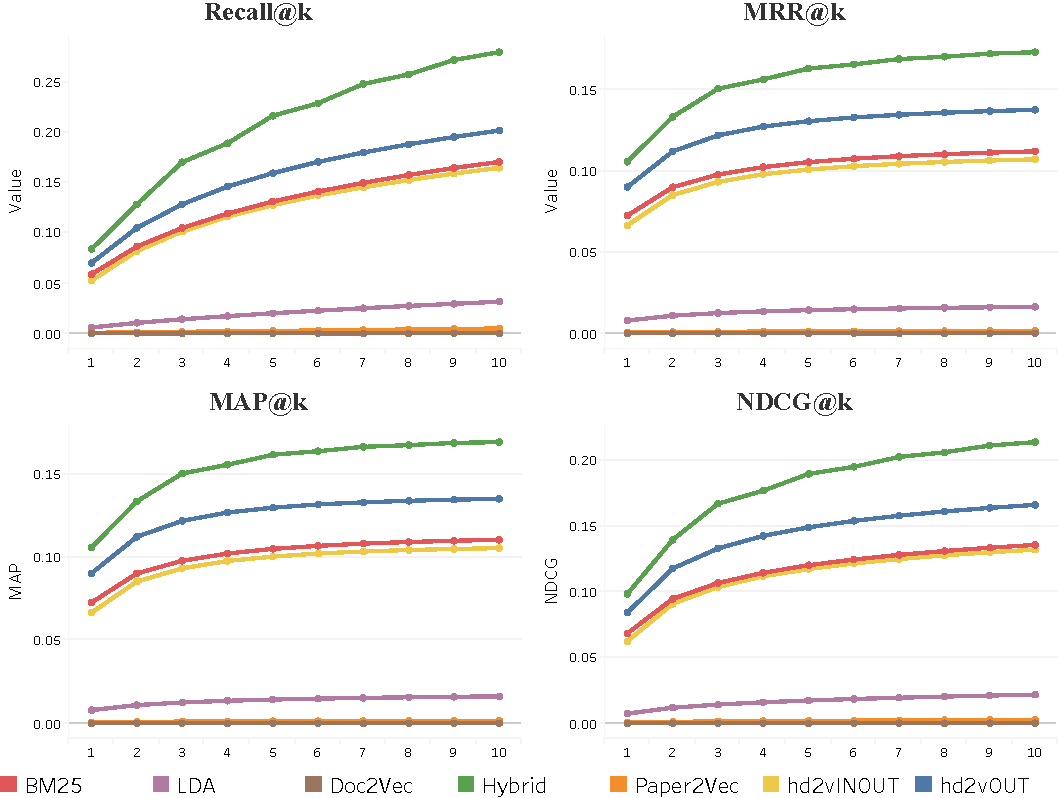
\includegraphics[keepaspectratio, width=.9\linewidth]{figures/Evaluation/ArxivMetricGraphs.pdf}
    \caption{Evaluation using Arxiv-MAG}
    \label{fig:arxivmagevaluation}
\end{figure}
\begin{figure}
    \centering
    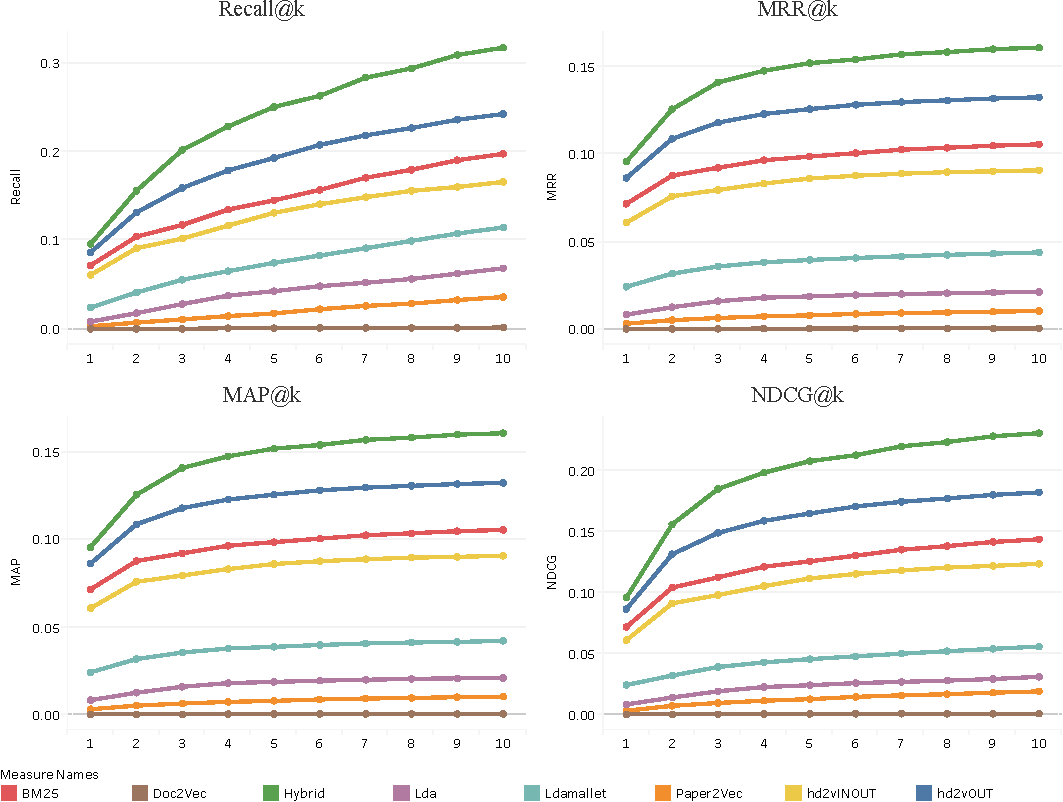
\includegraphics[keepaspectratio, width=.9\linewidth]{figures/Evaluation/ACLMetricGraphs.pdf}
    \caption{Evaluation using ACL-MAG}
    \label{fig:aclmagevaluation}
\end{figure}
Moving on to ACL-MAG, which has a very low number of test set contexts, we notice a few common patterns in Figure~\ref{fig:aclmagevaluation}. Using every metric, the performance of hd2vOUT is better than BM25, which is closely followed by hd2vINOUT. This reinforces the point made while analysing the Arxiv evaluation results that the IN document embeddings are better when some papers have full text.

Here, we also introduce a new LDA Mallet model in the results, which uses Gibbs sampling. This is said to be a better version of the Variational Bayes variant used with the other data sets, and the evaluation results bear that out. As pointed out earlier, the run time for LDA Mallet prediction is forbiddingly high. The considerable gap between LDA Mallet and the better algorithms in the graphs and the high execution time were the reasons why it wasn't used for the other data sets. 
The higher MAP and MRR when compared with MAG may simply be because of the sheer difference in size of the test sets.
\begin{figure}
    \centering
    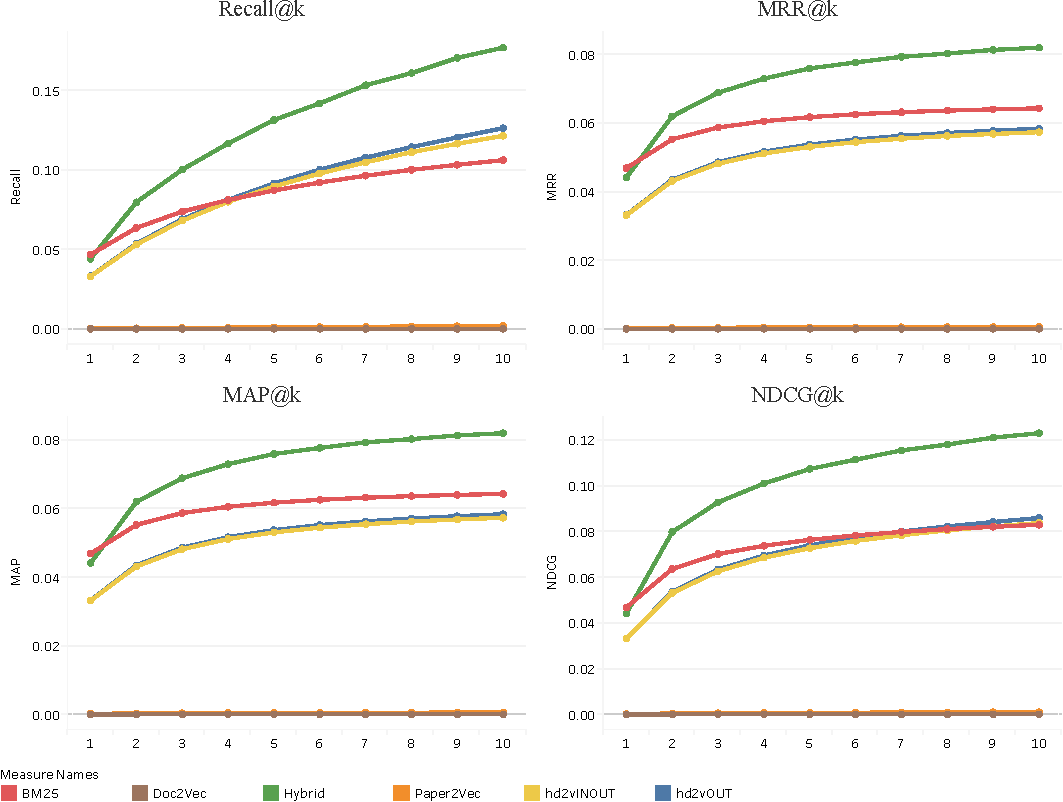
\includegraphics[keepaspectratio, width=.9\linewidth]{figures/Evaluation/UnpaywallMetricsGraph.pdf}
    \caption{Evaluation using Unpaywall-MAG}
    \label{fig:unpaywallmagevaluation}
\end{figure}
Lastly, we compare Unpaywall-MAG with Arxiv-MAG. The hd2vOUT and hd2vINOUT curves are very close to each other across metrics in the Unpaywall-MAG evaluation, but the concrete values are much lower than those for Arxiv-MAG. However, the recall rises more steeply with k for Unpaywall-MAG compared to Arxiv-MAG. The explanation for this might be that the same MAG test set is used for Unpaywall-MAG and the number of ground truths with more than one paper is not high. 

The low evaluation scores indicate that in general, the quality of embeddings for Unpaywall-MAG might be much lower than the Arxiv-MAG and MAG data sets. This is the reason all the algorithms (including BM25) do so much worse on Unpywall-MAG data than on the Arxiv-MAG and MAG data. This might be a signal that the conversion of PDF into XML using Grobid might have introduced some noise.  

At the end of the offline recommendation phase, we see a clear hierarchy in the performance of the algorithms across data sets and evaluation metrics. The hybrid algorithm performs the best and the two components of the hybrid algorithm, hd2vOUT and BM25 are the second and third best. There are some metrics and data sets for which BM25 performs better than hd2vOUT and some metrics and data sets for which it is the other way around. This is followed by hd2vINOUT and LDA. The other embedding algorithms, Paper2Vec and Doc2Vec, perform very badly. \\
As our main focus is on the MAG data sets, the online phase will use only the MAG data set, and the evaluation will be done for only the top 3 algorithms: Hybrid, BM25 and hd2vOUT.
\section{User Study and Online evaluation}
While the offline evaluation gives us an idea about how well the recommendation algorithms works, it does not paint the whole picture. Despite restricting test citation contexts from MAG to those with at least nine words (excluding stop words), it is entirely feasible that many of the contexts are too general to make any worthy recommendations. It is also possible that the citation contexts are noisy -- it might contain just formulae for example. 

This is reason enough to carry out a user study where a user manually rates the recommendations for a number of citation contexts using three algorithms: hd2vOUT, BM25 and the hybrid algorithm. It is important to note that Hybrid23 is not included in the user study. The reason for this is that we have restricted the user study to the best algorithms which work on a single data set. The user study is carried out only for the MAG data set (with no restriction on the number of citations) and is explained below.

The first step is the selection of a test set. Citation contexts are extracted from the MAG based on language and field of study. English citation contexts are chosen from the Natural Language Processing field as it closely relates to the topic of the thesis. All the citation contexts are chosen from 2018 and 2019. To make sure these contexts were seen in the offline evaluation test set, contexts which cite papers not from the training set are discarded. Duplicate contexts are grouped together. Additionally, citation contexts with 8 or fewer words (stop words not included) are discarded. 
\begin{figure}
    \centering
    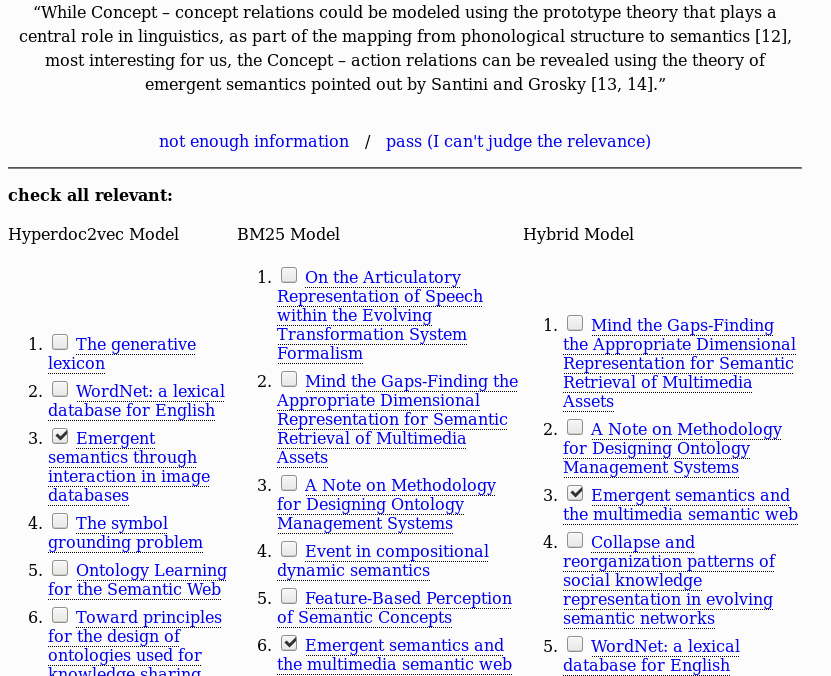
\includegraphics[keepaspectratio, width=.8\linewidth]{figures/Evaluation/userstudyinterface.PNG}
    \caption{User Study interface for example citation context}
    \label{fig:userstudyinterface}
\end{figure}
From the 8356 surviving citation contexts, random sampling is done to pick 100 citation contexts for the user study. 10 recommendations are made for each of these 100 citation contexts using each of the three chosen algorithms. The corresponding metadata -- title, abstract and the published year-- are retrieved from the MAG database. 
The recommendations, coupled with the metadata from MAG, are inserted in a JSON file. 

A web interface reads in these recommendations, and allows the user to select all the papers which are valid recommendations. The titles of the recommended papers are provided, with the corresponding abstracts in a tooltip. If the user can't understand the citation well enough to find suitable recommendations, he can select the 'pass' option. If the user believes there is not enough information in the context for it to be possible for a valid recommendation to be made, he selects the 'not enough information' option.
The user interface is shown in Figure~\ref{fig:userstudyinterface} for an example context. Here, it can be seen that one paper each is marked as valid for each of the algorithms. It is the same recommendation made by BM25 at position 6 and the hybrid algorithm at position 3. Incidentally, the ground truth for the same citation context during the offline evaluation consisted of the same papers. The hybrid algorithm misses one of them in the top 10 results. 

It is important to note that the selection of the relevant papers by the user was done based on the citation context only. So in case of contexts which are too short/general to convey the type of paper the author wanted to cite, the user had no choice but to pick recommender papers which relate to the general concept(s) in the citation context. \\
At the end of the binary rating process, 19 contexts were passed/not rated. So the total number of contexts for the online evaluation is 81.

Once the rating process for all the papers using the three models is completed, the recommendations are converted into arrays containing the positions at which the relevant papers were found. So, there are three arrays containing the positions of the relevant items for each of the three models: bm25, hd2vOUT and hybrid. These arrays are converted into binary arrays of size 10 with the positions of the relevant papers changed to ones. For example, if for a context, BM25 recommends [5,7], the corresponding binary array is [0,0,0,0,1,0,1,0,0,0].

The number of relevant papers for a test citation context is unavailable, unlike in the offline evaluation process. Instead, an approximation is made. The number of relevant results is approximated to be the sum of the results returned by hd2vOUT and BM25. The reason for this approximation is that in a vast majority of cases, the valid results picked by the user for the hybrid algorithm were from the top 10 results of hd2vOUT and BM25. The two individual models often complement each other, and pick different results. In many cases, hd2vOUT was found to recommend more general results (for example survey papers and oft-cited papers), while BM25 was found to recommend more specific results . This approximation only affects the calculation of one metric -- recall.

Three metrics are reported for the online evaluation: MAP, MRR and Recall. The NDCG is not reported because the recommendations are binary and not graded.
The calculated metrics (with recall subject to the aforementioned approximation) are shown in Table~\ref{tab:onlineevalresults}. 

\begin{table}[]
    \centering
    \begin{tabular}{cccc}
        \toprule
         Model & MAP@10 & Recall@10 & MRR@10  \\
         \midrule
         hd2vOUT & 0.314 & 0.385 & 0.315 \\
         BM25 & 0.362 & 0.541 & 0.380  \\
         Hybrid & 0.370 & 0.680 & 0.411  \\
         \bottomrule
    \end{tabular}
    \caption{Online evaluation at k=10 for 3 models using the MAG data set}
    \label{tab:onlineevalresults}
\end{table}

These results indicate that BM25 plays a dominant role in the hybrid algorithm, and outperforms hd2vOUT. However, there are a number of caveats with the online evaluation. The number of test set contexts is very small. The selection of relevant papers by the user are subjective and the citation contexts are sometimes ambiguous. The recommendations were selected only from one small field of study of computer science -- natural language processing. It isn't clear if choosing one field of study for the user study is representative of all computer science papers. 

But despite all the caveats, the user study allows us to make a number of inferences. hd2vOUT sometimes recommended some general papers relating to the concepts or claims mentioned in the citation contexts. BM25, being a text-based algorithm, recommended more specific results. As a result, their combination in the hybrid algorithm tends to combine the best of both worlds. 

Another observation was that even recommendations which are not perfectly suitable ones for the citation context might still be interesting to the end user. There are sometimes papers which touch on the topic of the citation context, or survey papers about a related research topic that might be useful. This \textit{serendipity} is a hallmark of recommender systems in general, and it could help researchers discover new topics related to their research areas.

The user study also shows that there are a number of citation contexts for which no recommendations are possible. Finally, it confirms the belief from the offline evaluation that BM25 and such text-based information retrieval algorithms work as well or better on the citation recommendations task as more complex algorithms.

Finally, the results of the user study indicate that users of the HybridCite citation recommendation system should be given an option to remove popular papers (which they are already likely to know). The hybrid algorithm often recommended such general, popular papers because hd2vOUT recommended them. So the user has been given the option of only being recommended papers with 500 or fewer citations in the HybridCite recommemder system.